%LTeX: language=fr-FR
\documentclass{exam}
\usepackage{tasks}

\usepackage{amsmath,amssymb,amsfonts}
\usepackage{graphicx}
\usepackage{amsthm}
\usepackage[french]{babel}
\usepackage{enumitem}
\usepackage{currfile}
\usepackage{tikz}
\usetikzlibrary{babel,arrows.meta,calc}
\usepackage{tkz-base}
\usepackage{tkz-euclide}
\setlength{\parindent}{0cm}

\usepackage{multicol}

\pagestyle{empty}
\graphicspath{ {../../Images/} }
\input{\currfiledir ../def.tex}
\def \Document {Contrôle 2}

\usepackage{geometry}
\geometry{left=1.5cm, right=1.5cm, top=1.5cm, bottom=1.5cm}

\theoremstyle{definition}
\newtheorem{exercice}{Exercice}

\colorlet{sol}{blue!70!black}

% En-tête d'un sujet
\newcommand{\entete}[1]{%
\noindent{
\makebox[0pt][l]{\textbf{\Niveau}}%
\makebox[\textwidth][c]{\textbf{\Chapitre}}%
\makebox[0pt][r]{\textbf{\Document\ (#1) -- Correction}}
}
\vspace{4mm}
}

% Exercice 3 : construction de T + u + v
% #1 : T ; #2 : origine de u ; #3 : u ; #4 : origine de v ; #5 : v ; #6 : nom du point
\newcommand{\construction}[6]{%
\begin{tikzpicture}[baseline={(current bounding box.north)}, scale=0.32]
\tkzInit[xmin=-9.9, xmax=9.9, ymin=-9.9, ymax=9.9]
\tkzGrid[thin,color=lightgray]
\draw[line width=1, ->, >=stealth] #2 -- ++#3 node[midway, above right] {$\vec{u}$};
\draw[line width=1, ->, >=stealth] #4 -- ++#5 node[midway, left] {$\vec{v}$};
\draw[sol, line width=1, dashed, ->, >=stealth] #1 -- ++#3 node[midway, sloped, above] {\small$\vec{u}$};
\draw[sol, line width=1, dashed, ->, >=stealth] ($#1+#3$) -- ++#5 node[midway, sloped, above] {\small$\vec{v}$};
\draw[sol, line width=1.5, ->, >=stealth] #1 -- ($#1+#3+#5$);
\draw[line width=1] plot[mark=x, mark size=0.2cm] coordinates{#1};
\node[above right] at #1 {$T$};
\draw[sol, line width=1] plot[mark=x, mark size=0.2cm] coordinates{($#1+#3+#5$)};
\node[sol, below right] at ($#1+#3+#5$) {$#6$};
\end{tikzpicture}%
}

% Exercice 4 : figure corrigée
% #1 : u ; #2 : v ; #3 : coefficient k (BP = k u, QR = -k u) ; #4 : texte de k
\newcommand{\figureABC}[4]{%
\begin{tikzpicture}[scale=0.8]
  \draw[gray!30,very thin,step=0.5] (0,0) grid (14,9);
  \coordinate (u) at #1;
  \coordinate (v) at #2;
  \coordinate (A) at (8,8);
  \coordinate (B) at ($(A)+(u)+(v)$);
  \coordinate (C) at ($(A)+(u)-(v)$);
  \coordinate (P) at ($(B)+#3*(u)$);
  \coordinate (Q) at ($(P)-2*(v)$);
  \coordinate (R) at ($(Q)-#3*(u)$);
  \draw[-{Latex[length=2.5mm]},thick] (4,7) -- ++(u) node[above left] {$\vec u$};
  \draw[-{Latex[length=2.5mm]},thick] (1,8) -- ++(v) node[above,midway] {$\vec v$};
  % Question 1
  \draw[-{Latex[length=2.5mm]},sol,dashed] (A) -- ++(u);
  \draw[-{Latex[length=2.5mm]},sol,dashed] ($(A)+(u)$) -- ++(v);
  \draw[-{Latex[length=2.5mm]},sol,dashed] ($(A)+(u)$) -- ++($-1*(v)$);
  \draw[-{Latex[length=2.5mm]},sol,very thick] (A) -- (B);
  \draw[-{Latex[length=2.5mm]},sol,very thick] (A) -- (C);
  % Question 2
  \draw[-{Latex[length=2.5mm]},red!70!black,very thick] (B) -- (P) node[midway, right] {$#4\vec u$};
  \draw[-{Latex[length=2.5mm]},red!70!black,very thick] (P) -- (Q) node[midway, below] {$-2\vec v$};
  \draw[-{Latex[length=2.5mm]},red!70!black,very thick] (Q) -- (R) node[midway, below right] {$-#4\vec u$};
  \foreach \p/\pos in {A/right, B/right, P/below right, Q/below left} {
    \node at (\p) {$\times$};
    \node[\pos] at (\p) {$\p$};
  }
  \node at (C) {$\times$};
  \node[above left] at (C) {$C = R$};
\end{tikzpicture}%
}

% Exercice 4 : question 3
% #1 : coefficient
\newcommand{\questionCR}[1]{%
On constate que les points $C$ et $R$ sont \textbf{confondus}.

\medskip
D'après la relation de Chasles :
\[
\overrightarrow{AR} = \overrightarrow{AB} + \overrightarrow{BP} + \overrightarrow{PQ} + \overrightarrow{QR}.
\]
Par construction :
\[
\overrightarrow{AR} = \left(\vec u + \vec v\right) + #1\vec u - 2\vec v - #1\vec u
= \vec u + \vec v - 2\vec v
= \vec u - \vec v.
\]
Or $\overrightarrow{AC} = \vec u - \vec v$, donc $\overrightarrow{AR} = \overrightarrow{AC}$ : les points $R$ et $C$ sont confondus.
}

\begin{document}
\large

%%%%%%%%%%%%%%%%%%%%%%%%%%%%%%%%%%%%%%%% SUJET A
\entete{A}

\begin{exercice}~\\
\begin{minipage}[t]{0.66\textwidth}%
\vspace{-\topskip}
\begin{enumerate}
    \item $ABCD$ est un parallélogramme, donc $\overrightarrow{BA} = \overrightarrow{CD}$.
    \[
    \overrightarrow{OC} + \overrightarrow{BA} = \overrightarrow{OC} + \overrightarrow{CD} = \overrightarrow{OD}.
    \]
    (On accepte aussi $\overrightarrow{BO}$, $\overrightarrow{EA}$ ou $\overrightarrow{CF}$.)
    \item Soustraire un vecteur, c'est ajouter son opposé : $-\overrightarrow{FD} = \overrightarrow{DF}$.
    \[
    \overrightarrow{ED} - \overrightarrow{FD} + \overrightarrow{AE}
    = \overrightarrow{AE} + \overrightarrow{ED} + \overrightarrow{DF}
    = \overrightarrow{AF}.
    \]
    (On accepte aussi $\overrightarrow{EC}$.)
\end{enumerate}
\end{minipage}
\begin{minipage}[t]{0.34\textwidth}%
\vspace{-\topskip}
\begin{center}
    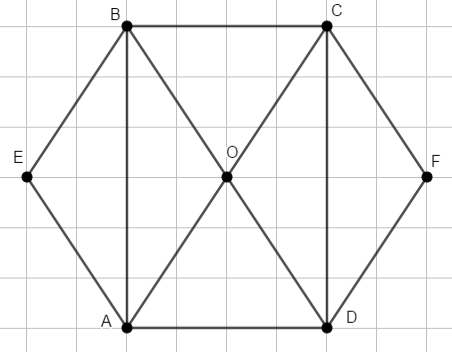
\includegraphics[width=0.95\linewidth]{cflash_7.png}
\end{center}
\end{minipage}
\end{exercice}

\begin{exercice}~
\begin{enumerate}
    \item $\overrightarrow{IP} + \overrightarrow{MI} = \overrightarrow{MI} + \overrightarrow{IP} = \overrightarrow{MP}$.
    \item $\overrightarrow{JI} - \overrightarrow{JK} + \overrightarrow{IK}
    = \overrightarrow{JI} + \overrightarrow{IK} - \overrightarrow{JK}
    = \overrightarrow{JK} - \overrightarrow{JK}
    = \vec{0}$.
\end{enumerate}
\end{exercice}

\begin{exercice}~\\
On trace $\vec u$ à partir de $T$, puis $\vec v$ à partir de l'extrémité de $\vec u$.

\medskip
\begin{minipage}[t]{0.5\linewidth}
\begin{center}
\construction{(-5,5)}{(-5,5)}{(7,-5)}{(-5,5)}{(4,-9)}{R}
\end{center}
\end{minipage}%
\begin{minipage}[t]{0.5\linewidth}
\begin{center}
\construction{(-2,0)}{(0,3)}{(4,-9)}{(3,1)}{(0,5)}{D}
\end{center}
\end{minipage}
\end{exercice}

\newpage

\begin{exercice}~
\begin{center}
\figureABC{(-3,-3)}{(2.5,0)}{1/3}{\frac{1}{3}}
\end{center}

\begin{enumerate}[label=\arabic*.]
    \item Pour $B$ : on trace $\vec u$ à partir de $A$, puis $\vec v$. Pour $C$ : on trace $\vec u$ à partir de $A$, puis $-\vec v$ (même direction que $\vec v$, sens contraire).
    \item $\dfrac{1}{3}\vec u$ a la même direction et le même sens que $\vec u$, et une longueur trois fois plus petite. $-2\vec v$ a la même direction que $\vec v$, le sens contraire et une longueur deux fois plus grande.
    \item \questionCR{\frac{1}{3}}
\end{enumerate}
\end{exercice}

\newpage

%%%%%%%%%%%%%%%%%%%%%%%%%%%%%%%%%%%%%%%% SUJET B
\setcounter{exercice}{0}
\entete{B}

\begin{exercice}~\\
\begin{minipage}[t]{0.66\textwidth}%
\vspace{-\topskip}
\begin{enumerate}
    \item $ABCD$ est un parallélogramme, donc $\overrightarrow{CD} = \overrightarrow{BA}$.
    \[
    \overrightarrow{OB} + \overrightarrow{CD} = \overrightarrow{OB} + \overrightarrow{BA} = \overrightarrow{OA}.
    \]
    (On accepte aussi $\overrightarrow{CO}$, $\overrightarrow{BE}$ ou $\overrightarrow{FD}$.)
    \item Soustraire un vecteur, c'est ajouter son opposé : $-\overrightarrow{FC} = \overrightarrow{CF}$.
    \[
    \overrightarrow{EC} - \overrightarrow{FC} + \overrightarrow{BE}
    = \overrightarrow{BE} + \overrightarrow{EC} + \overrightarrow{CF}
    = \overrightarrow{BF}.
    \]
    (On accepte aussi $\overrightarrow{ED}$.)
\end{enumerate}
\end{minipage}
\begin{minipage}[t]{0.34\textwidth}%
\vspace{-\topskip}
\begin{center}
    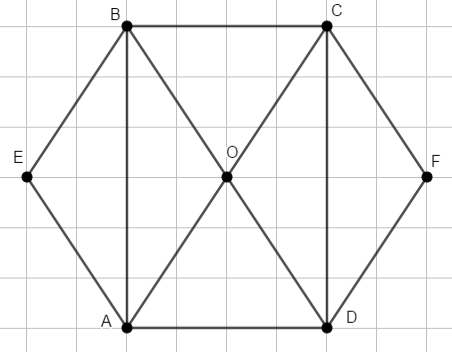
\includegraphics[width=0.95\linewidth]{cflash_7.png}
\end{center}
\end{minipage}
\end{exercice}

\begin{exercice}~
\begin{enumerate}
    \item $\overrightarrow{MN} + \overrightarrow{OM} = \overrightarrow{OM} + \overrightarrow{MN} = \overrightarrow{ON}$.
    \item Soustraire un vecteur, c'est ajouter son opposé : $-\overrightarrow{SU} = \overrightarrow{US}$.
    \[
    \overrightarrow{RU} + \overrightarrow{ST} - \overrightarrow{SU}
    = \overrightarrow{RU} + \overrightarrow{US} + \overrightarrow{ST}
    = \overrightarrow{RT}.
    \]
\end{enumerate}
\end{exercice}

\begin{exercice}~\\
On trace $\vec u$ à partir de $T$, puis $\vec v$ à partir de l'extrémité de $\vec u$.

\medskip
\begin{minipage}[t]{0.5\linewidth}
\begin{center}
\construction{(5,-5)}{(5,-5)}{(-3,5)}{(5,-5)}{(-6,1)}{R}
\end{center}
\end{minipage}%
\begin{minipage}[t]{0.5\linewidth}
\begin{center}
\construction{(-2,0)}{(0,3)}{(4,-9)}{(-3,1)}{(0,5)}{D}
\end{center}
\end{minipage}
\end{exercice}

\newpage

\begin{exercice}~
\begin{center}
\figureABC{(-3,-3)}{(2.5,0)}{1/3}{\frac{1}{3}}
\end{center}

\begin{enumerate}[label=\arabic*.]
    \item Pour $B$ : on trace $\vec u$ à partir de $A$, puis $\vec v$. Pour $C$ : on trace $\vec u$ à partir de $A$, puis $-\vec v$ (même direction que $\vec v$, sens contraire).
    \item $\dfrac{1}{3}\vec u$ a la même direction et le même sens que $\vec u$, et une longueur trois fois plus petite. $-2\vec v$ a la même direction que $\vec v$, le sens contraire et une longueur deux fois plus grande.
    \item \questionCR{\frac{1}{3}}
\end{enumerate}
\end{exercice}

% \newpage

% \begin{exercice}~
% \begin{center}
% \figureABC{(-2,-2)}{(3,0)}{1/2}{\frac{1}{2}}
% \end{center}
% 
% \begin{enumerate}[label=\arabic*.]
%     \item Même méthode qu'à l'exercice 4.
%     \item $\dfrac{1}{2}\vec u$ a la même direction et le même sens que $\vec u$, et une longueur deux fois plus petite.
%     \item \questionCR{\frac{1}{2}}
% \end{enumerate}
% \end{exercice}
% 
\end{document}
